% IEEE standard conference template; to be used with:
%   spconf.sty  - LaTeX style file, and
%   IEEEbib.bst - IEEE bibliography style file.
% --------------------------------------------------------------------------

\documentclass[letterpaper]{article}
\usepackage{spconf,amsmath,amssymb,graphicx,xspace,tabularx,hyperref}
\usepackage{cleveref}
\let\cref=\Cref % Capitalise `Section 3` etc. when referencing
\crefname{figure}{fig.}{figs.}
\crefname{algocf}{algorithm}{algorithms}
\usepackage[sort&compress,numbers,sectionbib]{natbib}
\usepackage[ruled,noalgohanging]{algorithm2e}
\usepackage{comment}
\input macros/todo
\input macros/macros

% bold paragraph titles
\newcommand{\mypar}[1]{{\bf #1.}}

% Title.
% ------
\title{A Descriptive Title, not too general, not too long}
%
% Single address.
% ---------------
\name{Henry Trinh, Richard Hladik, Stephanie Ruhstaller, Sarah Tr\"ondle}
\address{Department of Computer Science\\ ETH Zurich, Switzerland}

% For example:
% ------------
%\address{School\\
%		 Department\\
%		 Address}
%
% Two addresses (uncomment and modify for two-address case).
% ----------------------------------------------------------
%\twoauthors
%  {A. Author-one, B. Author-two\sthanks{Thanks to XYZ agency for funding.}}
%		 {School A-B\\
%		 Department A-B\\
%		 Address A-B}
%  {C. Author-three, D. Author-four\sthanks{The fourth author performed the work
%		 while at ...}}
%		 {School C-D\\
%		 Department C-D\\
%		 Address C-D}
%

\begin{document}
%\ninept
%
\maketitle
%

\begin{abstract}
	\templatecomment{Describe in concise words what you do, why you do it (not necessarily
in this order), and the main result. The abstract has to be
self-contained and readable for a person in the general area. You
	should write the abstract last.}
\end{abstract}

\section{Introduction}\label{sec:intro}
\begin{comment}
Do not start the introduction with the abstract or a slightly modified
version. What follows is a possible structure of the introduction.
This structure can be modified, but the content should be the same. The introduction should definitely end on the first page.

\mypar{Motivation} The first task is to motivate what you do.  You can
start general and zoom in one the specific problem you consider.  In
the process you should have explained to the reader: what you are doing,
why you are doing, why it is important (order is usually reversed).

For example, if my result is the fastest DFT implementation ever, one
could roughly go as follows. First explain why the DFT is important
(used everywhere with a few examples) and why performance matters (large datasets,
realtime). Then explain that fast implementations are very hard and
expensive to get (memory hierarchy, vector, parallel).

\mypar{Contribution}
Now you state what you do in this paper. In our example:
presenting a DFT implementation that is
faster for some sizes than all the other ones.

\mypar{Related work} Next, you have to give a brief overview of
related work. For a paper like this, anywhere between 2 and 8
references. Briefly explain what they do. In the end contrast to what
you do to make now precisely clear what your contribution is.
\end{comment}

\mypar{Motivation}
In the age of digitalization a majority of the people spend their time on different platforms for entertainment, online-shopping and other fields. With the number of items increasing tremendously, the consumer is challenged to choose a small set of items that meets his interests and preferences. To tackle this problem, recommender systems were invented. Since recommender systems play a big role in e-commerce profitwise, many companies have an incentive creating recommender systems that are accurate, robust, scalable and fast. However, these characteristics are hard to fulfill with incomplete, uncertain, inconsistent and/or intentionally contaminated data. Further, since new data keeps coming in frequent intervals, collaborative filtering techniques like \emph{Matrix Factorization}\rh{would not capitalise} require solving the entire problem again and impose computational limitations for large-scale deployment.\rh{paragraph break here?} \citet{BPRS} and \citet{top-n-recommendation} propose a different approach where the relation of the users and items are represented as graphical models. The idea is to calculate the marginal probability distribution of the nodes which corresponds to predicting the ratings of the items for users. Since computing the marginal probablity is intractable in general, they opted to approximate it with the \emph{belief propagation} (BP) algorithm which also\rh{why also?} grows linearly with the number of nodes (users/items) and therefore does not have the computational constraint such as the matrix factorization algorithm.

Many papers about BP focus on the algorithmic site for optimization. Our focus is a fast and efficient C implementation of the BP that takes into account the memory hierarchy and vectorization.

\mypar{Contribution}
We provide a BP implementation based on \citet{top-n-recommendation}. On top of that we optimize the performance by some algorithmic changes, standard C optimization techniques that include unrolling loops and scalar replacement, decreasing memory storage\rh{memory usage/footprint sounds better to me} and utilizing SIMD instructions. Our optimized version beats the baseline implementation and also the library \emph{libDAI} BP implementation \cite{libdai}. Our overall speedup is up to 500 times evaluated on the MovieLens datasets \cite{movieLens}.

\mypar{Related Work}
BP also have usage\rh{awkward phrasing IMO, ``BP is also used in decoders''?} as decoders for polar codes. For better performance, \citet{related1} propose an efficient early termination scheme based on convergence properties of \emph{log-likelihood ratio} messages of BP polar decoders. They showed that for 30 iterations, they effectively reduce the number of iterations by 72.6\%.\rh{don't understand. now I read this as ``so they use 30 iteration, which is 72.6\% less than before``, is that right?}

There are also works that focus on parallelization. \citet{related2} show one of the first parallel designs for BP with the Message Passing Interface paradigm, while \citet{related3} describe novel approaches to parallel message computation in BP using GPU parallelization.

In this paper, we focus on single core performance where we do not concern ourselves with the convergence properties of BP and only consider running the algorithm for a fixed number of iterations.


\section{Belief Propagation/Top-N Recommendation}\label{sec:background}

In this section, we briefly touch upon the general idea behind belief
propagation algorithms and formally define the variant that is at the heart of
our algorithm.

\todo[inline]{one paragraph about general belief propagation}

\mypar{Belief propagation} For the purpose of this article, we use \emph{belief
propagation} to refer to the algorithm of \citet[Section
2.1]{top-n-recommendation}, which we describe in the following paragraphs.

The input of the algorithm is a bipartite\rh{it is, but it isn't important to
the algorithm} undirected graph $G = (V, E)$. Each of the vertices $v\in V$ can
be in one of $S$ \emph{states}, labeled $x_1, \ldots, x_S \in X$. There is a
joint probability mass function $p: X^V \to [0, 1]$ (assumed intractable and
inaccessible to us) that captures the probability of each possible assignment of
states to vertices. The goal of the algorithm is, for each vertex $v_i$, to
calculate its marginal distribution $p_i: X \to [0, 1]$, i.e.:
%
$$p_i(x_j) = \sum_{\ves \in X^V: s_i = x_j} p(\ves) = \Pr_p[s_i = x_j]$$
%
% In other words, we want to know how probable it is that $v_i$ ends up in the respective states $\in X$.
To model $p$, the algorithm is also given a collection of node potentials
$\{\,\phi_i\,\}_{i \in V}, \phi_i: X \to [0, 1]$, and a collection of edge
potentials $\{\,\psi_{ij}\,\}_{ij \in E}, \psi_{ij}: X\times X \to [0, 1]$.
Intuitively, node potentials capture our priors about which states each vertex
inclines to, while the edge potentials capture the influence the state of a
vertex has on the state of its neighbours.\rhinline{now it's kind of fuzzy,
saying ``potentials SOMEHOW MAGICALLY model $p$'', without really saying how.
But I don't want to go into too much detail.}

\mypar{Message passing} The belief propagation algorithm itself consists of two
procedures: \emph{propagation} and \emph{belief calculation}.

\emph{Propagation} happens for a predefined number of iterations. For each vertex $i$, and each its neighbour $j$, we compute a \emph{message} $m_{ij} : X \to \Rpos$ as follows:
%
$$m_{ij}(x_c) = \sum_{x_d \in X} \nodepot_i(x_d)\edgepot_{ij}(x_d, x_c) \cdot \prod_{k \in N(i) \setminus j} m_{ki}(x_d)$$
%
Initially, all messages are set to all-ones, i.e.~$m_{ij}(\cdot) = 1$.

This can be directly expressed in pseudocode:

% Buggy links, so a dirty fix
\def\lineAlgoPropagateForI{4}
\def\lineAlgoPropagateCalcProduct{9}
\begin{algorithm}
\caption{One propagation step}
\label{algo:propagate}
\KwIn{$G = (V, E), \{\,\nodepot_i\,\}_{i \in V}, \{\,\edgepot_{ij}\,\}_{ij \in E}$}
\KwOut{$\{\,m'_{ij}\,\}_{ij \in E}$}
\algodefaults
	$m_{ij}(x) \leftarrow 1\mkern 20mu\forall ij \in E, x \in X$\;
	\For{$\text{iter} = 0, \ldots, \mathcal{I}$}{
		Swap $m$ and $m'$.\;
		\ShowLn\For{$i \in V$}{
			\For{$j \in N(i)$}{
				\For{$x_c \in X$}{
					$m'_{ij}(x_c) \leftarrow 0$\;
					\For{$x_d \in X$}{
						\ShowLn$M^d_j \leftarrow \prod_{k \in N(i) \setminus j} m_{ki}(x_d)$
						$m'_{ij}(x_c) \pluseq \nodepot_i(x_d)\edgepot_{ij}(x_d,x_c) M^d_j$
					}
				}
			}
		}
	}
\end{algorithm}

%Faster algo: add $\prod_{k \in N(i) \setminus j} m_{ki}(x_d)$

%$$C(V, E) = 11n + 4 \cdot \sum_{v\in V} \deg(v)^2\;\ge\;11n + 4m^2 / n$$

Give a short, self-contained summary of necessary
background information on the algorithm or application that you then later optimise including a cost analysis.

For example, assume you present an
implementation of FFT algorithms. You could organize into DFT
definition, FFTs considered, and cost analysis. The goal of the
background section is to make the paper self-contained for an audience
as large as possible. As in every section
you start with a very brief overview of the section. Here it could be as follows: In this section
we formally define the discrete Fourier transform, introduce the algorithms we use
and perform a cost analysis.

\mypar{Discrete Fourier Transform}
Precisely define the transform so I understand it even if I have never
seen it before.

\mypar{Fast Fourier Transforms}
Explain the algorithm you use.

\mypar{Cost Analysis}
First define you cost measure (what you count) and then compute or determine on other ways the
cost as explained in class. In the end you will likely consolidate it into one number (e.g., adds/mults/comparisons) but be aware of major imbalances as they affect the peak performance..

Also state what is known about the complexity (asymptotic usually)
about your problem (including citations).

% a few more ideas
\begin{itemize}
\item belief propagation how we explained in presentation (maybe generally state, what it is and mention that there are multiple ways of doing it, before giving our algorithm)
\item how to adapt it to make recommendations (just the sorting of the beliefs)
\item cost analysis from presentation
\end{itemize}


\section{Your Proposed Method}\label{sec:yourmethod}
\begin{figure}\centering
	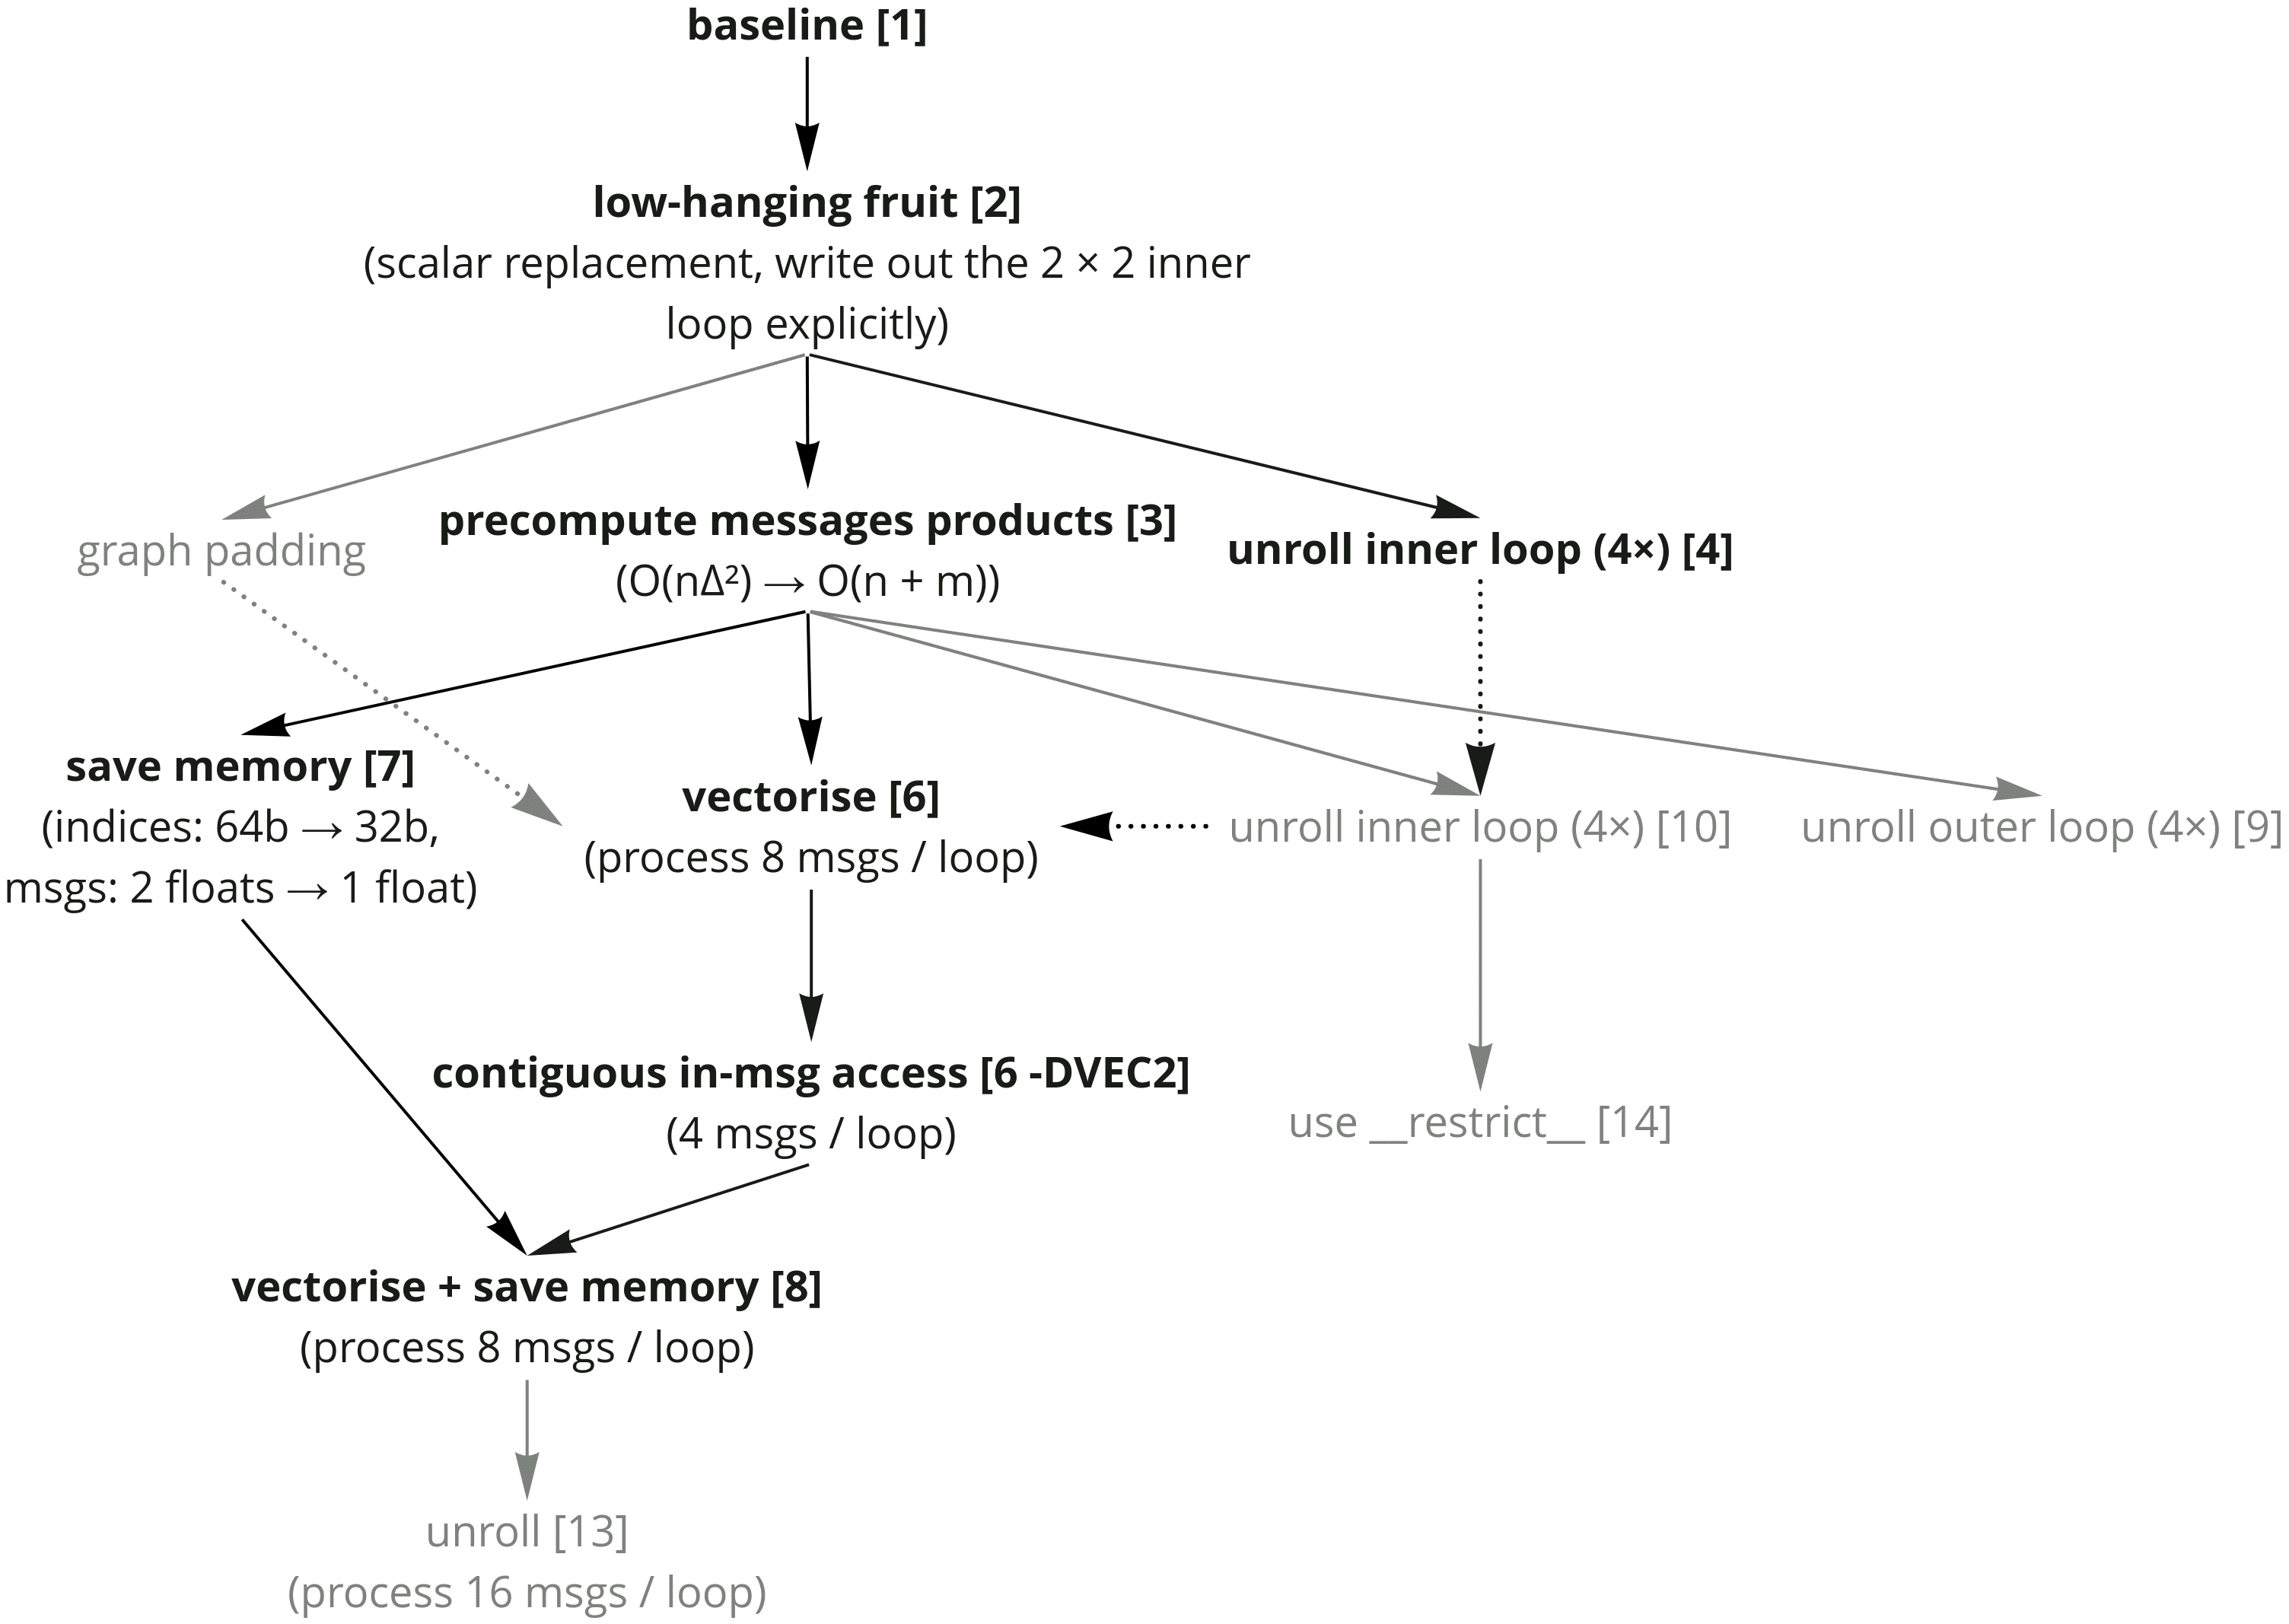
\includegraphics[width = 0.48 \textwidth]{img/OptimizationDiagram.png}
	\caption{Diagram of optimisation steps \label{OptDiagram}}
\end{figure}
\stinline{going to make the screen shot of the diagram prettier}

This section presents all optimization steps seen in figure TODO.
\todo[inline]{could be worth it to give number all optimization in the order they are presented in this section}

\mypar{Baseline [1]}
This project has two baselines. The first makes use of the C++ library libDAI, which implements belief propagation on a factor\rh{would drop the capitalisation} graph.
The second baseline, and basis for all optimization, was implemented from scratch and strictly follows the belief propagation algorithm presented in \cref{sec:background}. It was implemented in a way that tries to maximize sequential array access and uses a CSR (compressed sparse row) inspired format for storing incoming messages.

\mypar{Low-hanging fruit [2]}
The first optimizations applied on top of the baseline implementation were scalar replacement and writing out the inner two by two loops explicitly. \todo[inline]{reference lines in Algorithm 1} This optimization was then used as basis for all following steps.

Using scalar replacement for values that are accessed through pointers should allow the compiler to use more optimizations since the possibility of aliasing is excluded, and can possibly save memory accesses when a pointer is dereferenced once instead of multiple times.
Writing out the inner 2 by 2 loop saves on control flow instructions and besides saving computation, it also makes it more predictable for the compiler. \stinline{should the reasoning of our asumptions be in this section or in results?}
\HTinline{I think the reasoning for assumptions should be here since they are necessary to explain what and why we did this optimization. In the result, we'll have our plots that should validate those assumptions}
\rhinline{agree, although other way around it also kind of makes sense}


\mypar{Precompute message products [3]}
\rhinline{I plan on describing some of this in \cref{sec:background}, so I'll maybe move some of this there after I get to it.}
\stinline{good idea, then we can reference the theory like I did in the previous section}
In the next step the algorithm was optimized, specifically the message calculation. As seen in \cref{sec:background}, the messages get calculated according to:
$$m_{ij}(x_c) = \sum_{x_d \in X} \nodepot_i(x_d)\edgepot_{ij}(x_d, x_c) \cdot \prod_{k \in N(i) \setminus j} m_{ki}(x_d)$$
This means, that for every neighbor of a node computes a product of messages from all other neighbors of a node. To avoid repeating the same calculations, the product was replaced with the following:
$$\prod_{k \in N(i) \setminus j} m_{ki}(x_d) = \frac{1}{m_{kj}(x_d)} \cdot \prod_{k \in N(i)} m_{ki}(x_d)$$
Where $\prod_{k \in N(i)} m_{ki}(x_d)$ is the same for all neighbors of a node and therefore can be calculated in the outer loop. \todo[inline]{reference line of $i$-loop in algorithm 1}

This improves the asymptotic complexity of the belief propagation algorithm from $O(|E|\cdot avgDegree)$ to $O(|E|)$. Which means a drastic decrease in required flops per graph node, what should lead to a significant speedup.
\mypar{Unroll inner loop [4 \& 10]}
Unrolling the inner loop, the $j$-loop in \cref{algo:propagate}, was done once on basis of optimization 2 and once on basis of optimization 3. In both implementations, the loop was unrolled by a factor of 4. This allowed for more scalar replacement. Since the four loop iterations are independent, computing 4 iterations at once\rh{don't understand the ``combined'' here} \st{is it clearer now?} allows for more instruction level parallelism (ILP).
The difference in the two unrolling implementations is that thanks to optimization 2, the second version unrolls a loop with much fewer computations, which means that ILP can be expected to have less impact. But it should still clearly outperform the version with more flops.


\mypar{Unroll outer loop [9]}
In a different implementation\rh{would maybe mention that it's based on 2? but maybe having the tree figure is enough} we examined what happens if the outer loop is unrolled. Specially, the $i$-loop from \cref{algo:propagate} was unrolled by a factor of 4. Since with optimization 2 the product of old messages was pushed to the outer loop, it was of interest to see if unrolling this loop would allow for increased ILP. Or if, with 4 inner loops run during one unrolled iteration of the outer loop, the loss of locality would result in decreased performance.

\mypar{Graph padding}
In anticipation of unrolling and SIMD optional graph padding was added to optimization 3 and kept for all following optimisation steps (as seen in figure \ref{OptDiagram}.) The idea behind it was, to add additional nodes in the graph, that would not have any influence on the result, but would make the number of neighbors of a node divisible by 4 or 8 respectively. With this, when the j-loop from algorithm \ref{algo:propagate} is unrolled, there is no need to add a small left-over loop without unrolling. To see for every unrolling and vectorisation step, whether the additional nodes or the left-over loop are the bigger overhead, it was implemented with the help of macros. So the graph padding could easily be activated or deactivated.


\mypar{Vectorise [6]}
As seen in figure \ref{OptDiagram}, SIMD was introduced on basis of the message product precomputation. First, intel intrinsics for vector instructions were introduced, that very closely followed the instruction sequence of scalar computation. And 8 messages were processed together per loop iteration.

In a second step, the vector instructions were optimized with some shuffling to have more sequential access of the in-messages. Additionally, the number of messages handled during 1 iteration was reduced to 4. \st{maybe I should go into more detail here}

Even though, looking at the assembly compiled from optimization 2, it was visible that the compiler already introduced some vector instruction, writing them explicitly should allow for a greater use of SIMD.
\begin{comment}
For this course, explain all the optimisations you performed. This mean, you first very briefly
explain the baseline implementation, then go through locality and other optimisations, and finally SSE (every project will be slightly different of course). Show or mention relevant analysis or assumptions. A few examples: 1) Profiling may lead you to optimise one part first; 2) bandwidth plus data transfer analysis may show that it is memory bound; 3) it may be too hard to implement the algorithm in full generality: make assumptions and state them (e.g., we assume $n$ is divisible by 4; or, we consider only one type of input image); 4) explain how certain data accesses have poor locality. Generally, any type of analysis adds value to your work.

As important as the final results is to show that you took a structured, organized approach to the optimisation and that you explain why you did what you did.
\end{comment}

In a second step, the type of indices were changed from site\_t to uint\_32. This could be done, since the size of the data structures were knwon to never need more than 4 bytes to be indexed.

This compaction allowed for more values being read when loading 1 cache block. Making memory access more efficient.

\mypar{Combining vectorize and save memory [8]}
\begin{itemize}
\item combined the two
\item expect to work well, since with increasing computational efficiency memory accesses become a bigger bottleneck
\end{itemize}

\mypar{Unroll [13]}
\begin{itemize}
\item try to see what happens if unrolled more
\item more ILP or loss of locality?
\end{itemize}

\mypar{Use \_\_restrict\_\_ [14]}
\begin{itemize}
\item see if compiler can make use of additional information
\end{itemize}

%Now comes the ``beef'' of the paper, where you explain what you
%did. Again, organize it in paragraphs with titles. As in every section
%you start with a very brief overview of the section.
%
%For this course, explain all the optimizations you performed. This mean, you first very briefly
%explain the baseline implementation, then go through locality and other optimizations, and finally SSE (every project will be slightly different of course). Show or mention relevant analysis or assumptions. A few examples: 1) Profiling may lead you to optimize one part first; 2) bandwidth plus data transfer analysis may show that it is memory bound; 3) it may be too hard to implement the algorithm in full generality: make assumptions and state them (e.g., we assume $n$ is divisible by 4; or, we consider only one type of input image); 4) explain how certain data accesses have poor locality. Generally, any type of analysis adds value to your work.
%
%As important as the final results is to show that you took a structured, organized approach to the optimization and that you explain why you did what you did.
%
%Mention and cite any external resources including library or other code.
%
%Good visuals or even brief code snippets to illustrate what you did are good. Pasting large amounts of code to fill the space is not good.

%idea how we could structure this seciton
\begin{itemize}
\item maybe make a subsection for every field in the diagram, explain what we did and what we expected form it
\end{itemize}

\section{Experimental Results}\label{sec:exp}

%The effect of successful optimisations described in the previous section on performance and runtime are being evaluated in this section.
This section demonstrates the incremental performance and runtime improvements achieved by successively applying succeeding optimisations.  
We start with providing details about experimental setup first, then show the results of applying optimisations and finally show a roofline plot.
\srinline{Maybe mention ten iterations of propagate were performed and what instructions where used to measure the cycles and how we counted flops?}
\HTinline{Yeah, I would mention those things(added them at the end of experimental setup part)}
\mypar{Platform} All the experiments were conducted on the following setup:
\\
\begin{tabularx}{\linewidth}{ 
		>{\raggedright\arraybackslash}l
		>{\raggedright\arraybackslash}X 
	}
	\textbf{Processor}	&	Intel(R) Core(TM) i5-7200U														\\
	\textbf{Code name}	&	Kabylake \cite{intelSpec}														\\
	\textbf{Cores}		&	2 \cite{intelSpec}																\\
	\textbf{Threads}	&	4 \cite{intelSpec}																\\
	\textbf{Frequency} 	&	2.50GHz (Turbo Boost disabled)													\\
	\textbf{L1 cache} 	& 	2 x 32 KB 8-way set associative instruction cache \cite{optimisationManual}		\\
						&	2 x 32 KB 8-way set associative data cache \cite{optimisationManual}	 		\\
	\textbf{L2 cache}	&	2 x 256 KB 4-way set associative cache \cite{optimisationManual}				\\
	\textbf{L3 cache}	&	3 MB 12-way set associative shared cache \cite{cpuWorldSpec, intelSpec}			\\
	\textbf{RAM} 		&	2 × 8 GB DDR4 2133 MT/s 														\\
\end{tabularx}
\\
The processor specification states a maximum overall memory bandwidth of 34.1 GB/s for two channels \cite{intelSpec}.
Halving this number, gives 17.05 GB/s per channel.
In contrast, measuring the memory throughput of this platform for a single core using John D. McCalpin's STREAM memory benchmark gave the following results:
\\
\begin{tabularx}{\linewidth-5mm}{ 
		>{\raggedright\arraybackslash}X
		>{\raggedright\arraybackslash}X
	}
	\textbf{Function}	&	\textbf{Best Rate [MB/s]}	\\ \hline
	Copy 				&	14'273.6					\\
	Scale				&	13'646.1					\\
	Add 				&	16'250.3					\\
	Triad				& 	16'047.6 					\\
\end{tabularx}
\\
Taking the average over all functions gives 15'054.4 MB/s which is around 15 GB/s.
Dividing this 15 GB/s by 2.5 GHz, results thus in an average memory bandwidth $\beta=6$ bytes/cycle.

Further we use the \emph{RDTSC} instruction to measure the number of cycles. For the number of flops, we wrote a small code that counts the number of flops. In addition we let BP run for fixed amount of iterations, namely 10. \HT{maybe move 10 iterations somewhere else}

\mypar{Compiler} The program was compiled usig GCC 12.1.0 with 'g++ -Ofast -march=native'.

\mypar{Input data} Test inputs were based on the MovieLens dataset \cite{movieLens}.
Various sizes were generated by taking the ratings of users with identifier smaller than some number for different numbers
and then normalising / desparsifing the user and movie identifers seperately.
This section's plots display the results of either a small or a big dataset composed from inputs generated this way.
The small dataset represents graphs of 981 to 10,334 vertices and consists of inputs % 981, 1'879, 2'442, 3'128, 4'142, 4'847, 5'167, 5'879, 6'452, 7'272, 7'766, 8'522, 9'278, 10'334
considering the first 10, 20, 30, 60, 90, 120, 150, 210, 270, 330, 390, 450 and 540 users based on the small MovieLens dataset.
The big dataset represents graphs of 45,729 to 221,588 vertices and considers the first 16,200, 32,400 ... 162,000 (doubling the threshold everytime) users based on the full MovieLens dataset.

\mypar{Base implementation / optimisation} Since there are two base implementations, one implemented from scratch and the other using the libDAI library, it is interesting to see which one is slower.
For this purpose, the speedup in runtime of the different base implementations with respect to the from scratch implementation is displayed in \cref{libSpeedupSmall} on the small dataset.
We see that libDAI library [0] uses the most cycles compared to the others.
Already implementing the algorithm from scratch provided slight runtime benefits (baseline [1] in \cref{libSpeedupSmall}).
Presumably, this came from the benefits of not using a library: less bound checks and function calls / inlining of functions.
Another reason is that baseline [1] was implemented in a way to maximize sequential array access and used a CSR inspired format for storing all the incoming messages.
Appling optimisation [2] unrolling the two innermost loops of \cref{algo:propagate} iterating over the two states to the baseline [1] gives a 4x speedup.
A reason for this is that the product calculation at line nine of the algorithm could be reused by the outer loop iterating over states. \sr{*}
\begin{figure}\centering
	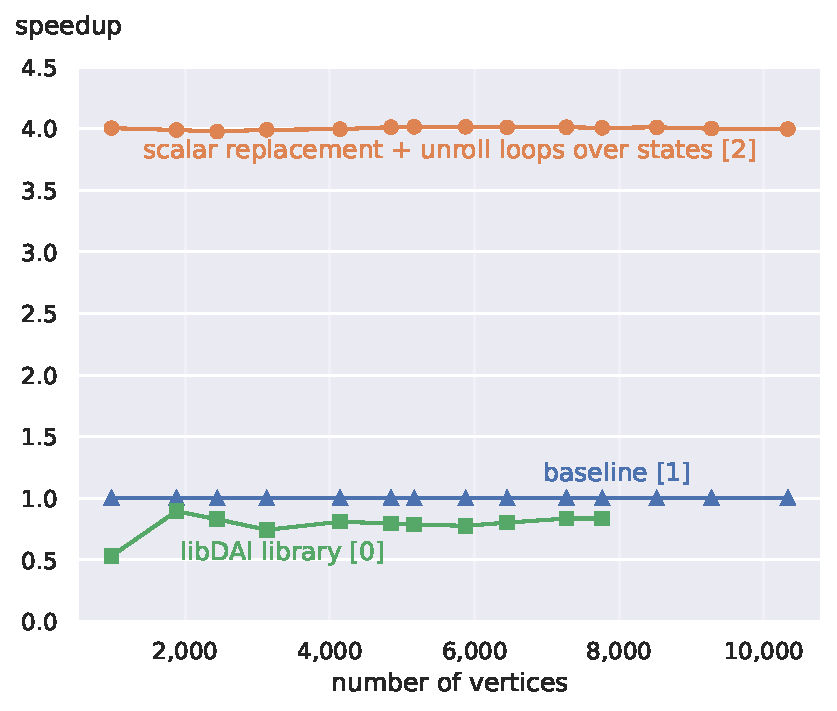
\includegraphics[scale=0.59]{img/speedup[0][1]_small.pdf}
	\caption{Speedup of optimisation step [2] over baseline [1] and libDAI library [0] with respect to the baseline on the small dataset. \label{libSpeedupSmall}}
\end{figure}

\mypar{Reducing computation} Optimisation [3] was applied on top of optimisation [2] and reduced floating point operations by replacing the computation of the product at line nine in \cref{algo:propagate} with a single division in addition to moving the product into the outermost loop.
How much of runtime improvement does optimisation step [3] achieve despite the fact that on the used platform less divisions can be scheduled per cycle than additions/multiplication and that they have a greater latency than additions/mulitplications \cite{optimisationManual}?
\cref{precomputeSpeedupSmall} shows that a speedup of at least 20x was achieved on the small dataset by this with respect to optimisation [2].
It seems that there were enough neighbours for each node to compute the product over.\sr{(?)*}
\begin{figure}\centering
	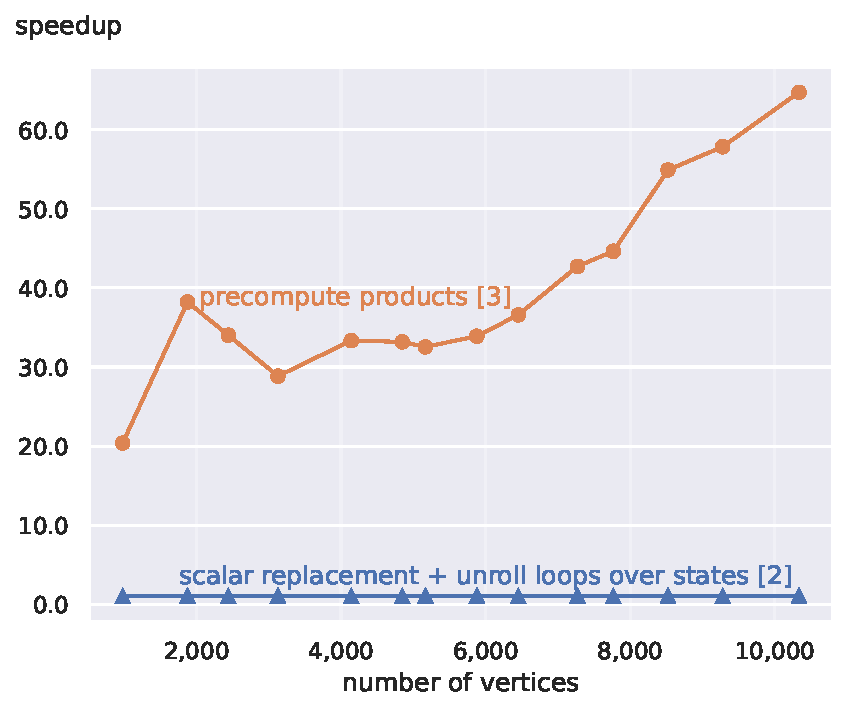
\includegraphics[scale=0.58]{img/speedup[2][3]_small.pdf}
	\caption{Speedup of optimisation step [3] (precomputing the product) added on top of optimisation [2] on the small dataset. \label{precomputeSpeedupSmall}}
\end{figure}
\srinline{Add a paragraph about graph padding, the nature of the test input (average degree in graph) and the effect of alignment? Include fully bipartite graph measurements?}
\HTinline{Yes and to the bipartite part, the plot should disprove the assumption that graph padding on higher degree graph helps}
\mypar{Saving memory and vectorisation} 
For further improvement on top of optimisation [3], one one hand optimisation [7] additionally tried to save memory and on the other hand optimisation [6] added vectorization.
How do these optimisations impact the speedup ?
We see in \cref{cpctVectSpeedupSmall} that for the small dataset there is only a speedup of around 1.1x with saving memory while vectorisation yields a speedup of at most 1.6x with respect to optimisation [3].
The speedup of the combined version of both optimisations (optimisation [8] in \cref{cpctVectSpeedupSmall}) is greather than each of them seperately.
\begin{figure}\centering
	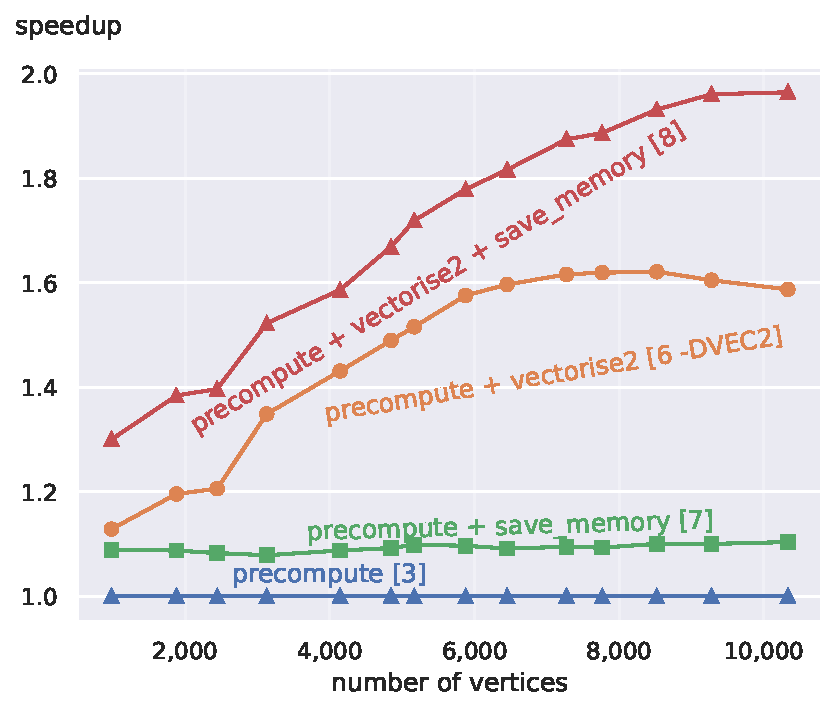
\includegraphics[scale=0.59]{img/speedup[3][6][7][8]_small.pdf}
	\caption{Speedup of vectorisation and saving memory optimisations based on optimisation [3] (precomputing the product) on the small dataset. \label{cpctVectSpeedupSmall}}
\end{figure}
Since the optimisations displayed in \cref{cpctVectSpeedupSmall} constitute the final steps taken and since we only discussed what happens on the small dataset so far, it is interesting to see the actual performance achieved and also how it changes for a working set that doesn't fit into cache anymore.
To this end, \cref{cpctVectPerformanceBoth} shows the performances of these optimizations on the small and big dataset combined.
We see that for the bigger inputs the combined version is still the best but the memory saving has a much bigger impact on speedup.
The vectorised versions drop faster than the nonvectorised versions as their advantages in efficient computation get drowned out by slow memory accesses.
All the opimisations displayed surpass the performances of the base implementions (mentionned in \cref{libSpeedupSmall}), whose performances were all below 0.1 flops/cycle.
For the versions saving memory, starting from the datapoint close to 50,000 vertices, the data structures didn't fit in to cache anymore.
\begin{figure}\centering
	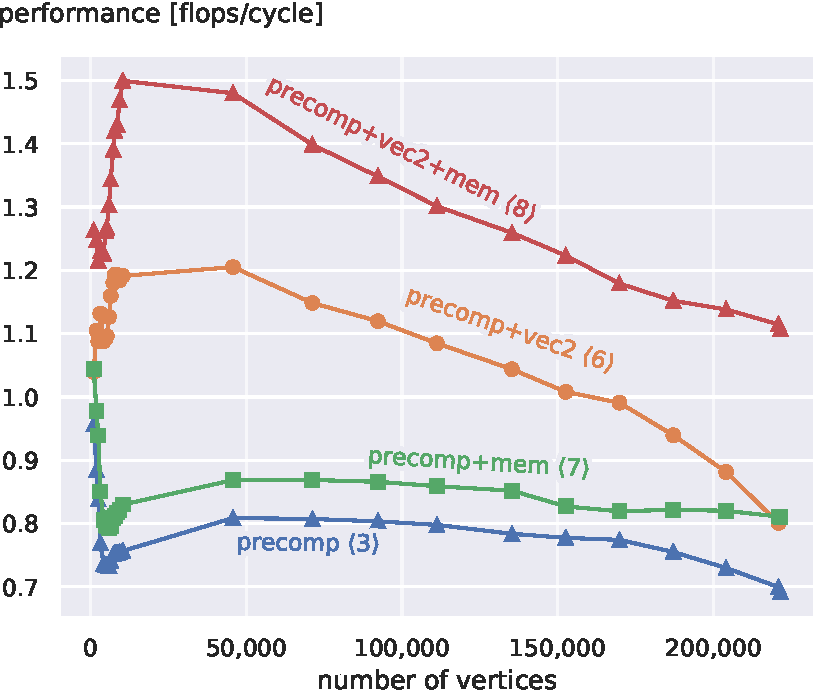
\includegraphics[scale=0.59]{img/performance[3][6][7][8]_both.pdf}
	\caption{Speedup of vectorisation and saving memory optimisations based on optimisation [3] (precomputing the product) on the small and big dataset combined. \label{cpctVectPerformanceBoth}}
\end{figure}

\mypar{Roofline}
Optimisation step [8] is the final one.
In order to see whether it is memory or compute bound and how close it is to the optimal performance consider \cref{rooflineEndToEndSmall}.
It obvious from \cref{rooflineEndToEndSmall} that all versions reside in the compute-bound region.
The last optimisation step achieves around 16.25\% of the vectorized peak performance and 65\% of the scalar peak performance on average on the platform.  
\begin{figure}\centering
	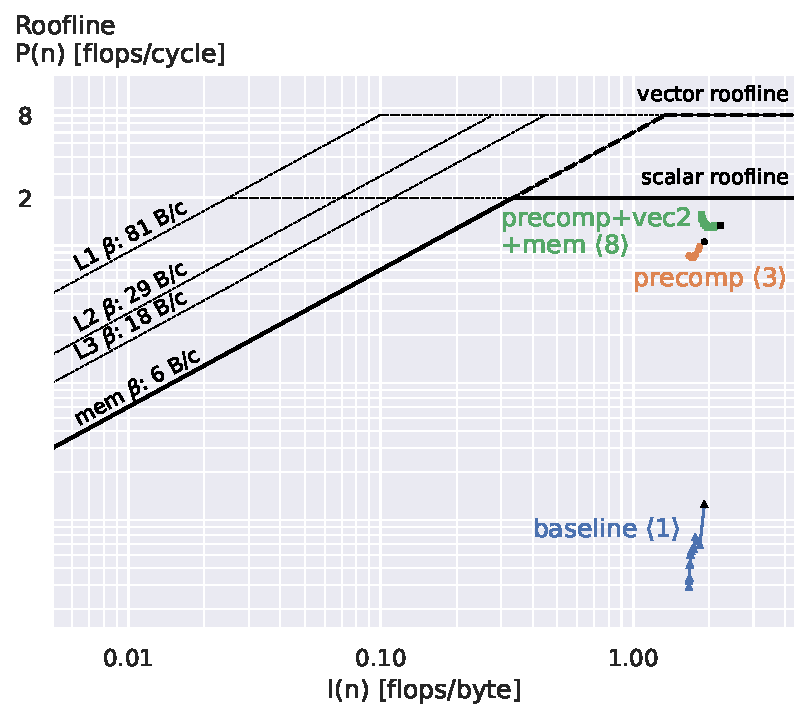
\includegraphics[scale=0.59]{img/roofline[1][3][8]_small.pdf}
	\caption{Roofline plot of optimisation steps [8], [3] (precompute products) and the baseline using the small dataset.
			\emph{The rooflines are with respect to scalar / vectorized peak processor performance (2 resp. 8 flops/cycle) and the bandwidth between L3 cache and memory ($\beta = 6$). } \label{rooflineEndToEndSmall}}
\end{figure}

\mypar{End-to-end speedup} To see the runtime gain achieved overall, \cref{speedupEndToEndSmall} displays the speedup on the small dataset.
The overall speedup lies between 100 to 500x for optimisation step [8].
Since optimisation step [3] was the last to have performed a major algorithmic optimisation, it is displayed for reference as well in \cref{speedupEndToEndSmall}.
\begin{figure}\centering
	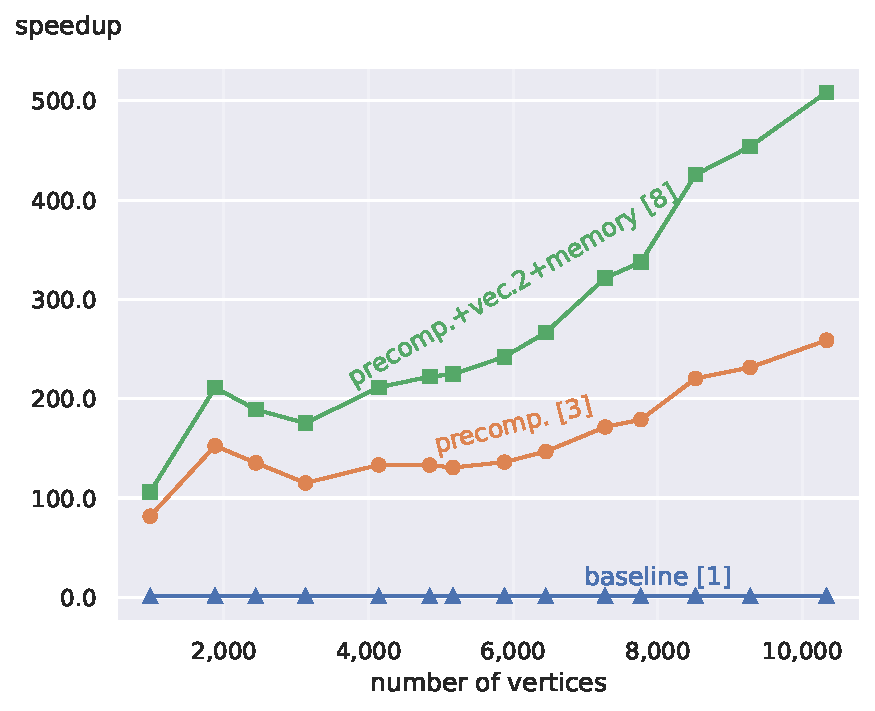
\includegraphics[scale=0.56]{img/speedup[1][3][8]_small.pdf}
	\caption{End-to-end speedup over baseline [1]. on the small dataset} \label{speedupEndToEndSmall}
\end{figure}

\srinline{Maybe use abbreviations in the plot e.g. prec, vec2, mem? Replot curves s.t. across plots the same color is used?}
\HTinline{good idea}
\srinline{Maybe a measurement of the baseline [1] on the big dataset would be beneficial for the roofline and end-to-end speedup?}
\HTinline{I think we should do it on big and small dataset for roofline + end-to=end speedup}
\srinline{What do you think?}

%Here you evaluate your work using experiments. You start again with a
%very short summary of the section. The typical structure follows.

%\mypar{Experimental setup} Specify the platform (processor, frequency, cache sizes)
%as well as the compiler, version, and flags used. I strongly recommend that you play with optimisation flags and consider also icc for additional potential speedup.

%Then explain what input you used and what range of sizes. The idea is to give enough information so the experiments are reproducible by somebody else on his or her code.

%\mypar{Results}
%Next divide the experiments into classes, one paragraph for each. In the simplest case you have one plot that has the size on the x-axis and the performance on the y-axis. The plot will contain several lines, one for each relevant code version. Discuss the plot and extract the overall performance gain from baseline to best code. Also state the percentage of peak performance for the best code. Note that the peak may change depending on the situation. For example, if you only do additions it would be 12 Gflop/s
%on one core with 3 Ghz and SSE and single precision floating point.

%Do not put two performance lines into the same plot if the operations count changed significantly (that's apples and oranges). In that case first perform the optimisations that reduce op count and report the runtime gain in a plot. Then continue to optimise the best version and show performance plots.

%{\bf You should}
%\begin{itemize}
%\item Follow to a reasonable extent the guide to benchmarking presented in class, in particular
%\item very readable, attractive plots (do 1 column, not 2 column plots
%for this class), proper readable font size. An example is below (of course you can have a different style),
%\item every plot answers a question, which you pose and extract the
%answer from the plot in its discussion
%\end{itemize}
%Every plot should be referenced and discussed (what does it show, which statements do
%you extract).

\section{Conclusions}

In this paper, we focused on implementing and optimising belief propagation for top-N-recommendation in C in a fast and efficient way.
Recommendation of products which a specific user might be interested in plays an important role on online shopping, video and streaming platforms nowadays. 
We achieved a 100 to 500x speedup on an Intel(R) Core(TM) i5-7200U and up to 16.25\% vectorized peak performance on a small dataset which fits into cache.
On a bigger dataset not fitting into the cache anymore, reducing the memory usage of data structures at the exchange of more computation had a bigger positive impact on speedup.
Also, for bigger inputs advantages in efficient computation get drowned out by slow memory access.
Out off all optimisation steps, replacing a product calculation with a division operation and moving the product to the outermost loop as an optimisation step achieved the greatest speedup.\sr{*}
There might be ways to further improve the performance our implementation since it is compute-bound and did not hit peak performance.\sr{*}
%Here you need to briefly summarize what you did and why this is
%important. {\em Do not take the abstract} and put it in the past
%tense. Remember, now the reader has (hopefully) read the paper, so it
%is a very different situation from the abstract. Try to highlight
%important results and say the things you really want to get across
%(e.g., the results show that we are within 2x of the optimal performance ...
%Even though we only considered the DFT, our optimisation
%techniques should be also applicable ....) You can also formulate next
%steps if you want. Be brief.


\section{Further comments}

Here we provide some further tips.

\mypar{Further general guidelines}

\begin{itemize}
\item For short papers, to save space, I use paragraph titles instead of
subsections, as shown in the introduction.

\item It is generally a good idea to break sections into such smaller
units for readability and since it helps you to (visually) structure the story.

\item The above section titles should be adapted to more precisely
reflect what you do.

\item Each section should be started with a very
short summary of what the reader can expect in this section. Nothing
more awkward as when the story starts and one does not know what the
direction is or the goal.

\item Do not use subsubsections.

\item Make sure you define every acronym you use, no matter how
convinced you are the reader knows it.

\item Always spell-check before you submit.

\item Be picky. When writing a paper you should always strive for 
high quality. Many people may read it and the quality makes a big difference.
In this class, the quality contributes to the grade.

\item Books helping you to write better: \cite{Higham:98} and \cite{Strunk:00}.
\end{itemize}

\mypar{Graphics} For plots that are not images {\em never} generate (even as intermediate step)
jpeg, gif, bmp, tif. Use eps, which means encapsulate postscript, or pdf. This way it is
scalable since it is a vector graphic description of your graph. E.g.,
from Matlab, you can export to eps or pdf.

\Cref{fftperf} is an example plot that I used in a lecture. Note that the fontsize in the plot should not be any smaller. On the other hand it is also a good rule that the font size in the plot is not larger than the one in the caption (otherwise it looks ugly).

\begin{figure}\centering
  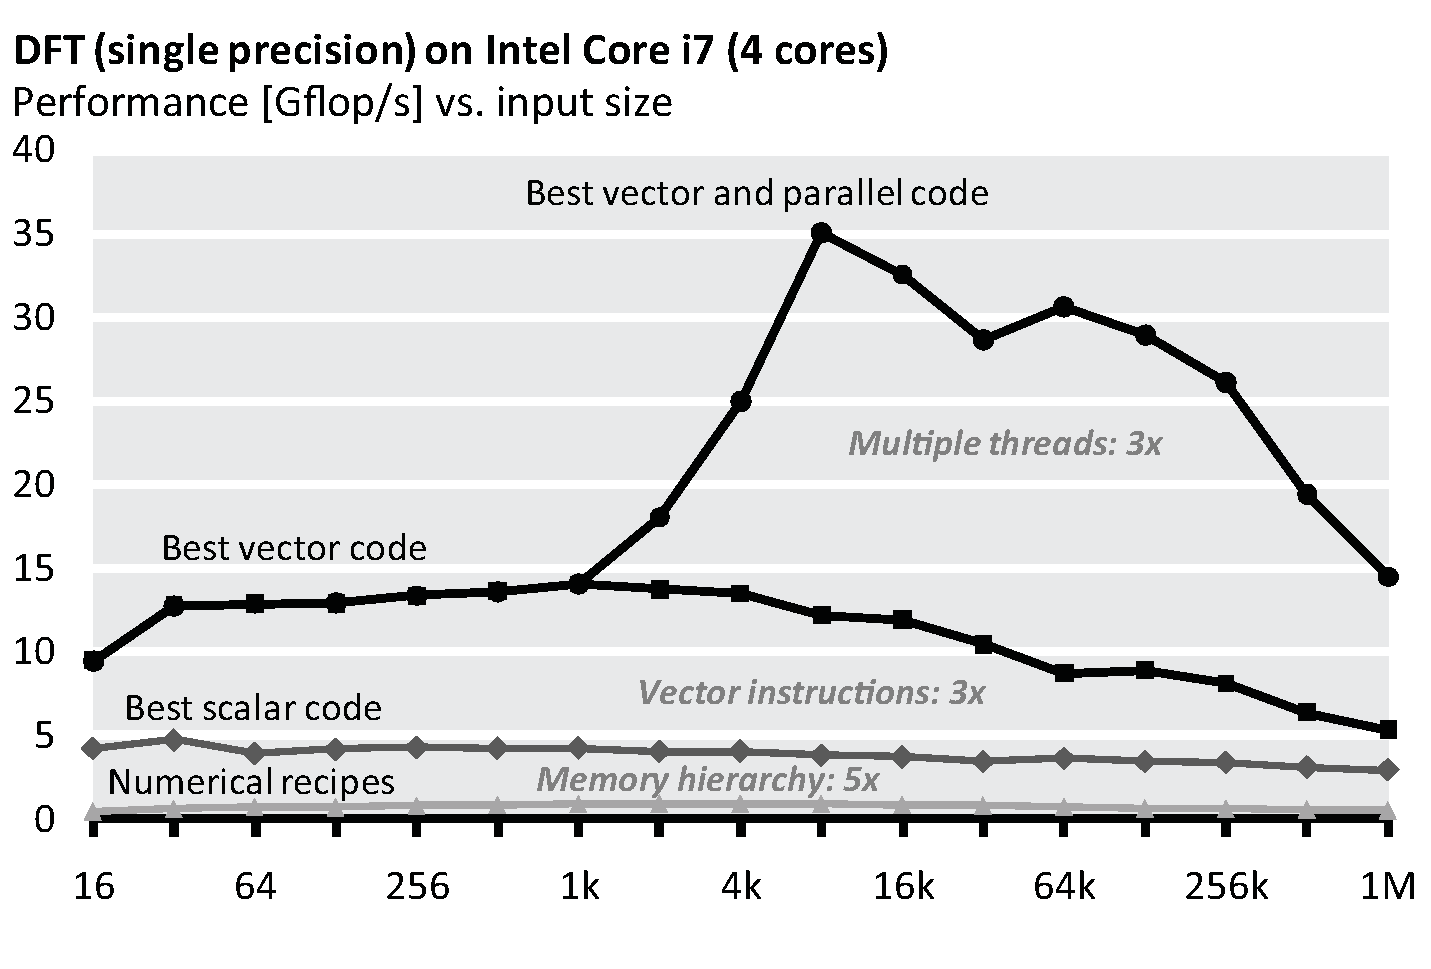
\includegraphics[scale=0.33]{img/dft-performance.pdf}
  \caption{Performance of four single-precision implementations of the
  discrete Fourier transform. The operations count is roughly the
  same. {\em The labels in this plot are about the smallest you should go.}\label{fftperf}}
\end{figure}

\bigskip
{\bf Up to here you have 8 pages.}

\section{Contributions}% of Team Members (Mandatory)

%In this mandatory section (which is not included in the 8 pages limit) each team member should very briefly (telegram style is welcome) explain what she/he did for the project. I imagine this section to be between one column and one page (absolute maximum).

%Include only 
%\begin{itemize}
%	\item What relates to optimising your chosen algorithm / application. This means writing actual code for optimisation or for analysis.
%	\item What you did before the submission of the presentation.
%\end{itemize}
%Do not include
%\begin{itemize}
%	\item Work on infrastructure and testing.
%	\item Work done after the presentation took place.
%\end{itemize}

%Example and structure follows.

\mypar{Richard} Did the base implementation from scratch in C in a favourable way maximizing sequential array access and using a CSR inspired format for storing incoming messages. Performed unrolling optimisation of innermost 2x2 loops over states and scalar replacement. Implemented precomputation of product optimisation. Helped Henry implementing/improving the roofline plot. Mostly prepared the slides on cost measure, experimental setup. Performed measurements and prepared plots.

\mypar{Henry} Implemented flop counting in code. Tried out unrolling outer loop over nodes further. Tried out unrolling inner loop over neighbours of a node further. Tried out log-domain opimisation turning products into summations. Extended flop counting with e.g. byte counting. Implemented roofline plot. Helped with preparing plots for the presentation, mainly the roofline.

\mypar{Sarah} Implemented flop counting in code of both algorithms together with Henry. Improved library flop counting. Performed unrolling optimisation of inner loop over neighbours of a node. Mostly prepared the slides on optimisations for the presentation.

\mypar{Stephanie} Did the base implementation using the libDAI library. Vectorized loop iterating over neighbours of a node. Implemented saving memory optimisation as discussed. Tried out restrict keyword and compiler flags. Mostly prepared slides on algorithm and cost measure for the presentation.

\srinline{Just wrote down what came into my mind so far. Most likely the description is incomplete and some points are wrong. Fix it.}

\section{Global TODOs}

\rhinline{just a list of TODOs we should tackle before submitting, feel free to add/disagree}
\todo[inline]{BrE vs AmE (RH has a script somewhere)}
\todo[inline]{spellcheck}
\todo[inline]{check there are no more TODOs hiding}
\todo[inline]{generally check the title, abstract, that we have no more template text somewhere}
\todo[inline]{minor details: use cref where appropriate, $\O$ instead of $O$, \texttt{xxx} instead of `xxx` etc.}

% References should be produced using the bibtex program from suitable
% BiBTeX files (here: bibl_conf). The IEEEbib.bst bibliography
% style file from IEEE produces unsorted bibliography list.
% -------------------------------------------------------------------------
%\bibliographystyle{IEEEbib}
\bibliographystyle{IEEEtranN}
\bibliography{bibliography}

\end{document}
